\chapter{Ďalšie výsledky inferencie modelov}\label{app:more-results}
V~tejto prílohe sú zobrazené ďalšie výsledky inferencie modelov \MC{}, \MCfim{} a nástoja GitHub Copilot na základe zvolených príkladov. Výsledky sú zobrazené vo forme obrázkov, ktoré zobrazujú zdrojový kód vygenerovaný modelmi pre zvolené príklady. Niektoré výsledky sú zobrazené v~porovnaní s~referenčným zdrojovým kódom, ktorý bol použitý na trénovanie modelov, prípadne šedou farbou sú zvýraznené časti kódu, ktoré boli modelom vygenerované. V~prípade \MC{} a GitHub Copilot dostal model iba textové zadanie a signatúru funkcie, zatiaľ čo vstup pre \MCfim{} je upravený spôsobom, ktorý som opísal v~sekcii~\ref{sec:microcoderfim-training}.

\section{MicroCoder}

Na obrázku~\ref{fig:mc-comp} je vidieť, že výsledky modelu \MC{} sa pre rovnaký vstup významne líšia. Kvantizácia váh má vplyv na \uv{zmätenosť} (angl. perplexity) modelu a tým aj na jeho schopnosť generovať zmysluplné výstupy. Niekedy model nevygeneruje nič zmysluplné, inokedy je výstup prínosný -- obrázok~\ref{fig:mc76.1}. Miera zmätenosti modelu sa zvyšuje s~klesajúcou bitovou hĺbkou modelu~\cite{llamaquant}. Na základe toho, že kvantizácia ovplyvňuje zmätenosť modelu, je dôležité posúdiť, či takáto optimalizácia je vhodná pre špecifické použitie modelu. Pri aplikáciách, kde je kritická vysoká presnosť a komplexnosť generovaného kódu, môže byť kvantizácia kontraproduktívna.

\begin{figure}[H]
    \centering
    \raisebox{-\height}{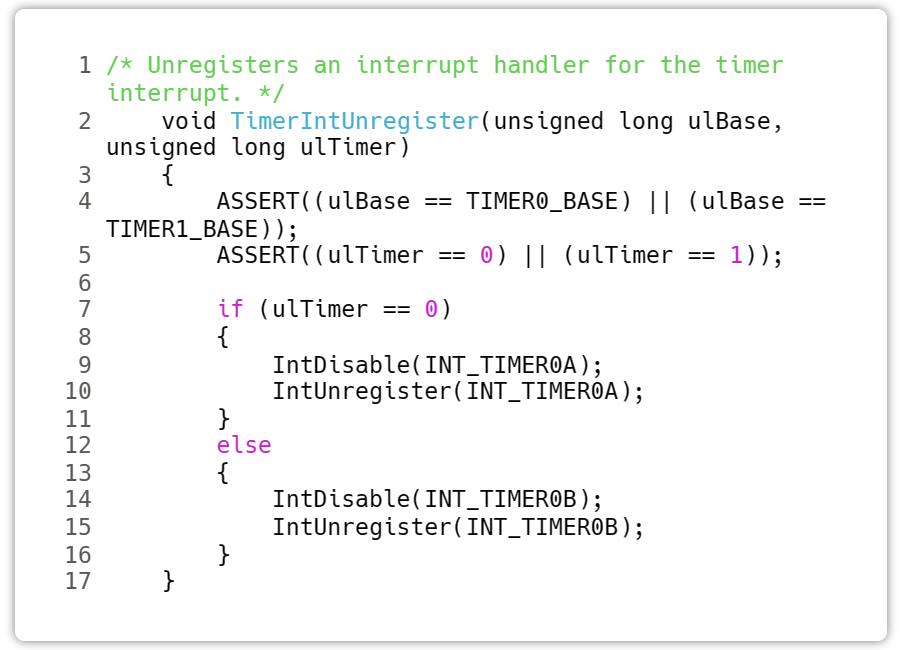
\includegraphics[width=0.45\textwidth]{obrazky/mc76.png}}
    \raisebox{-\height}{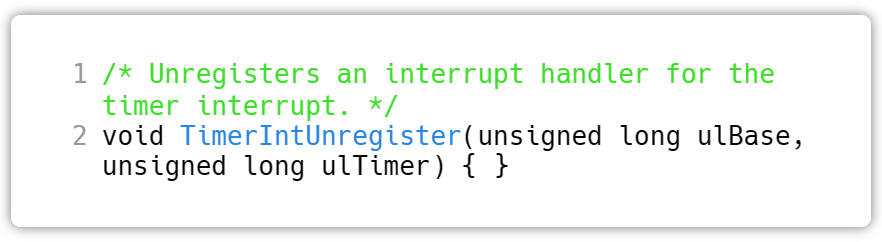
\includegraphics[width=0.45\textwidth]{obrazky/mc76.1.png}}
    \caption{Dva rôzne výstupy modelu \MC{} na rovnaký dotaz s~použitím rovnakých parametrov.}
    \label{fig:mc76.1}
\end{figure}

\begin{figure}[H]
    \centering
    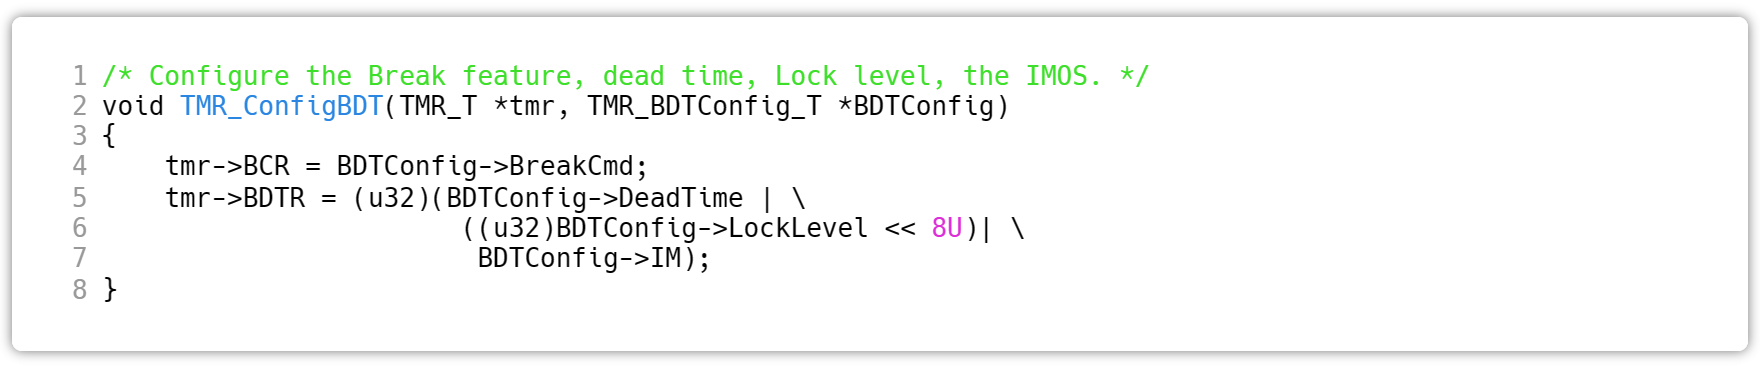
\includegraphics[width=1\textwidth]{obrazky/mc1.1.png}\\
    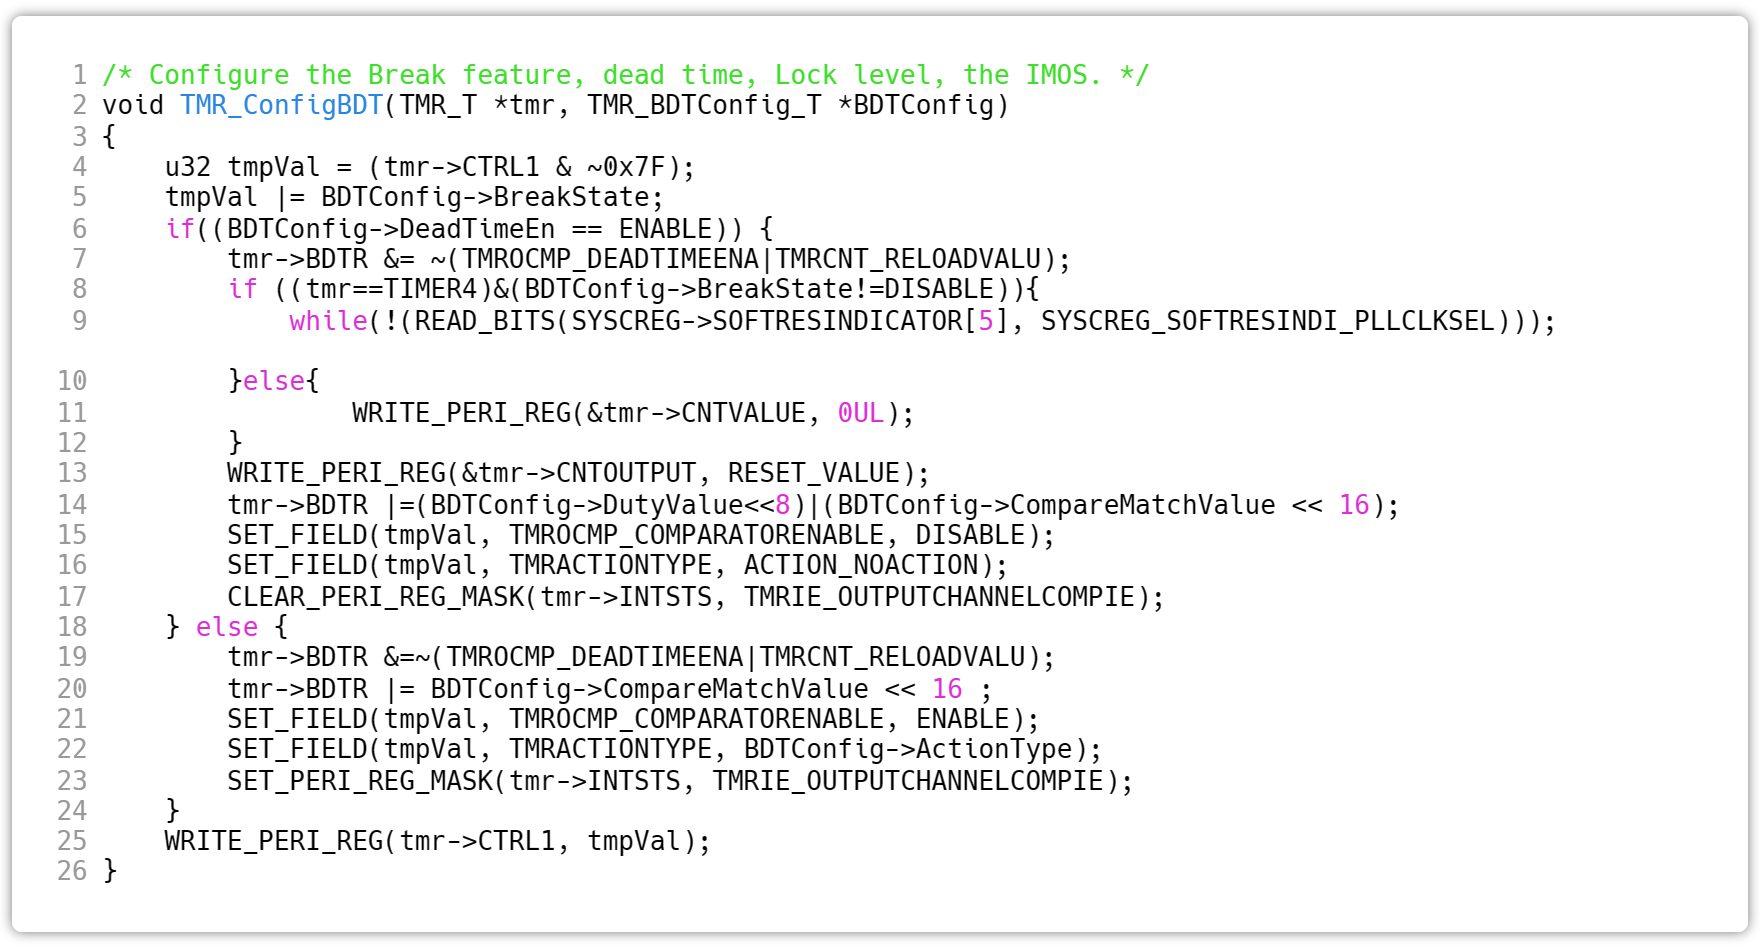
\includegraphics[width=1\textwidth]{obrazky/mc1.png}\\
    \caption{Dva rôzne výstupy modelu \MC{} na rovnaký dotaz s~použitím rovnakých parametrov. Na prvý pohľad je vidno, že dané výstupy sú veľmi odlišné. Prvý výstup (hore) je jednoduchší a priamočiarejší. Definuje dva hlavné príkazy pre nastavenie registra. Druhý výstup (dolu) je zložitejší, obsahuje viac vetvení a kontrolných štruktúr.}
    \label{fig:mc-comp}
\end{figure}

\begin{figure}[H]
    \centering
    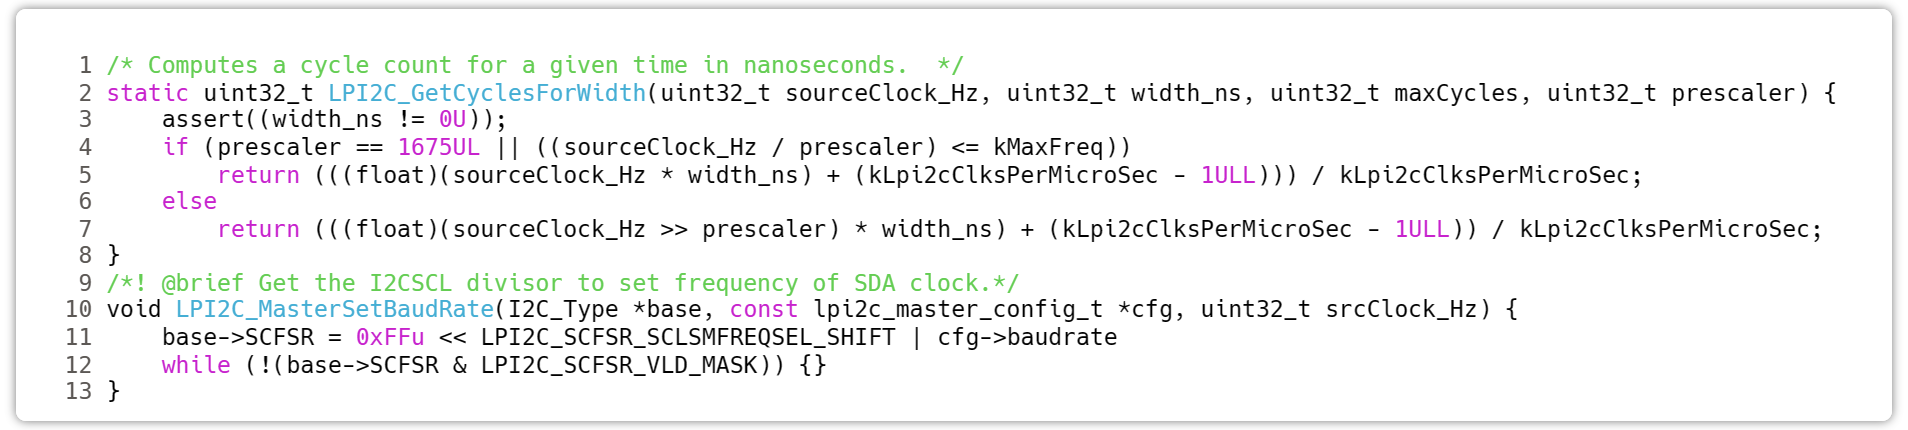
\includegraphics[width=1\textwidth]{obrazky/mc589.png}\\
    \caption{Výstup modelu \MC{}.}
    \label{fig:mc589}
\end{figure}

\section{Github Copilot}

\begin{figure}[H]
    \centering
    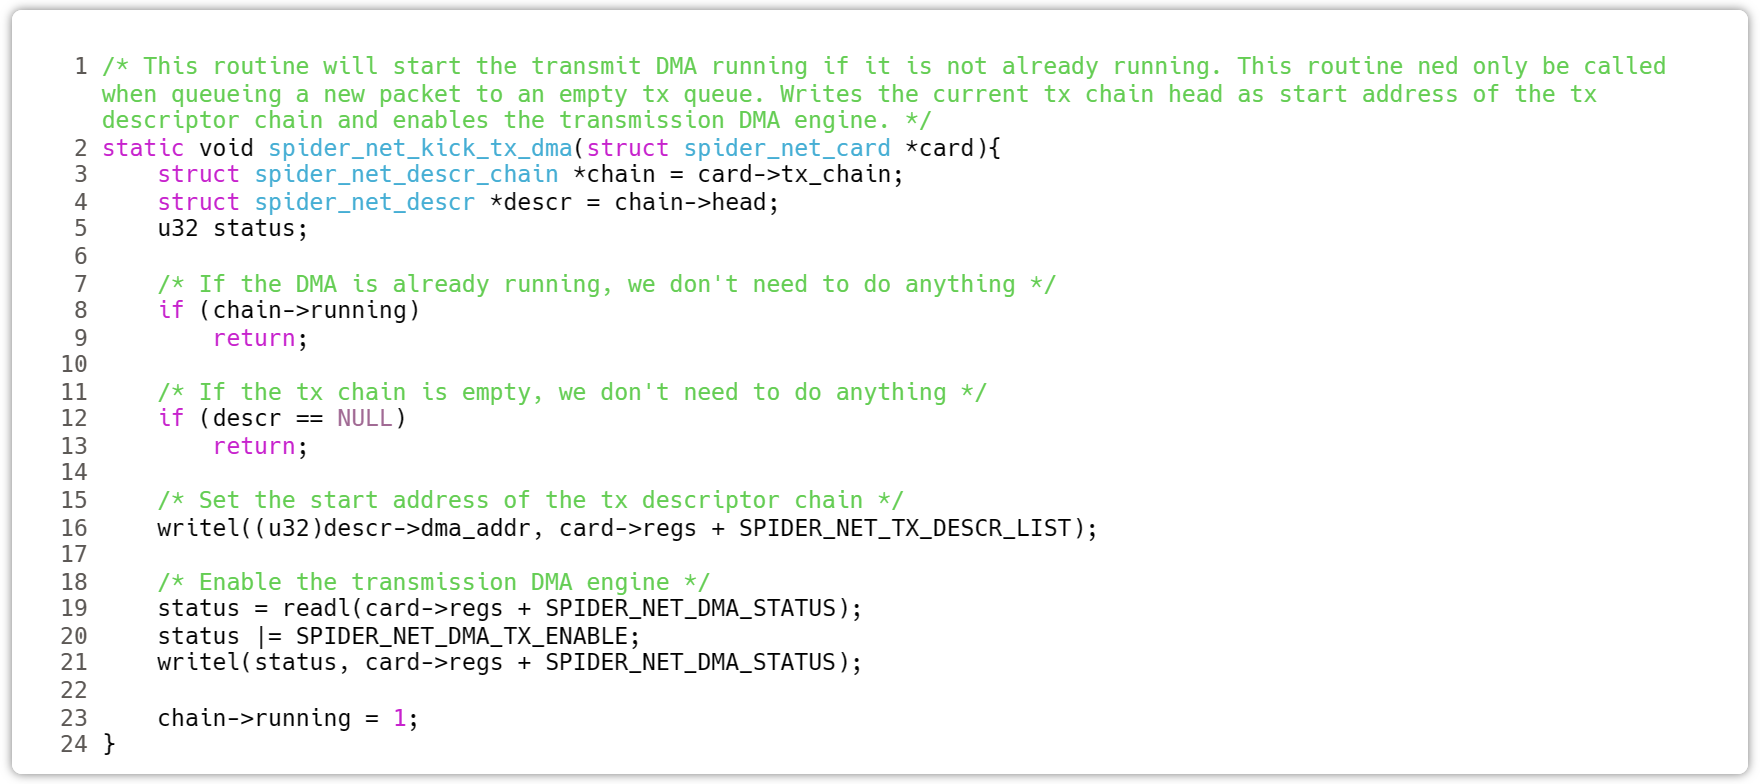
\includegraphics[width=1\textwidth]{obrazky/gpt1.png}
    \caption{Kód vygenerovaný nástrojom GitHub Copilot.}
    \label{fig:gpt1}
\end{figure}

\begin{figure}[H]
    \centering
    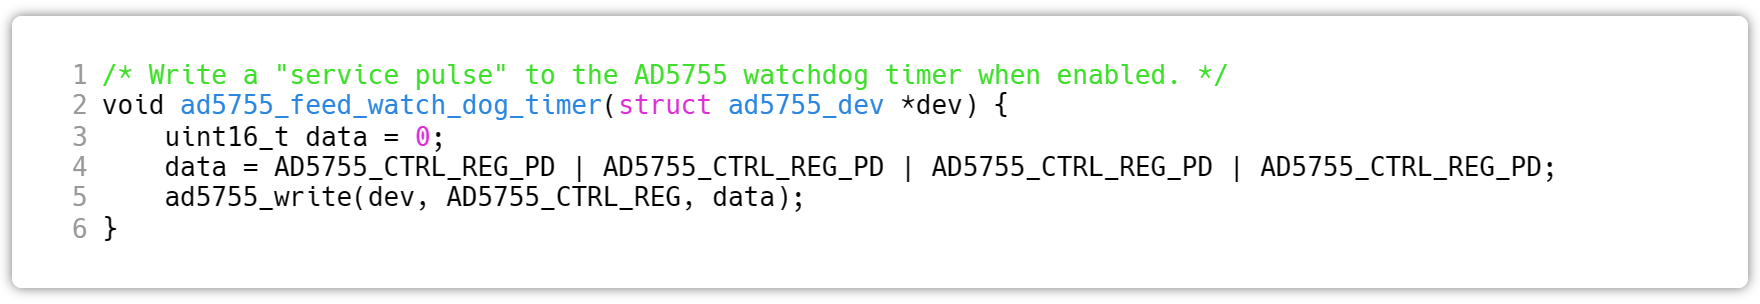
\includegraphics[width=1\textwidth]{obrazky/gpt2.png}
    \caption{Kód vygenerovaný nástrojom GitHub Copilot. Kód nebol vygenerovaný naraz, ale postupne na tri rôzne nápovedy.}
    \label{fig:gpt2}
\end{figure}

\begin{figure}[H]
    \centering
    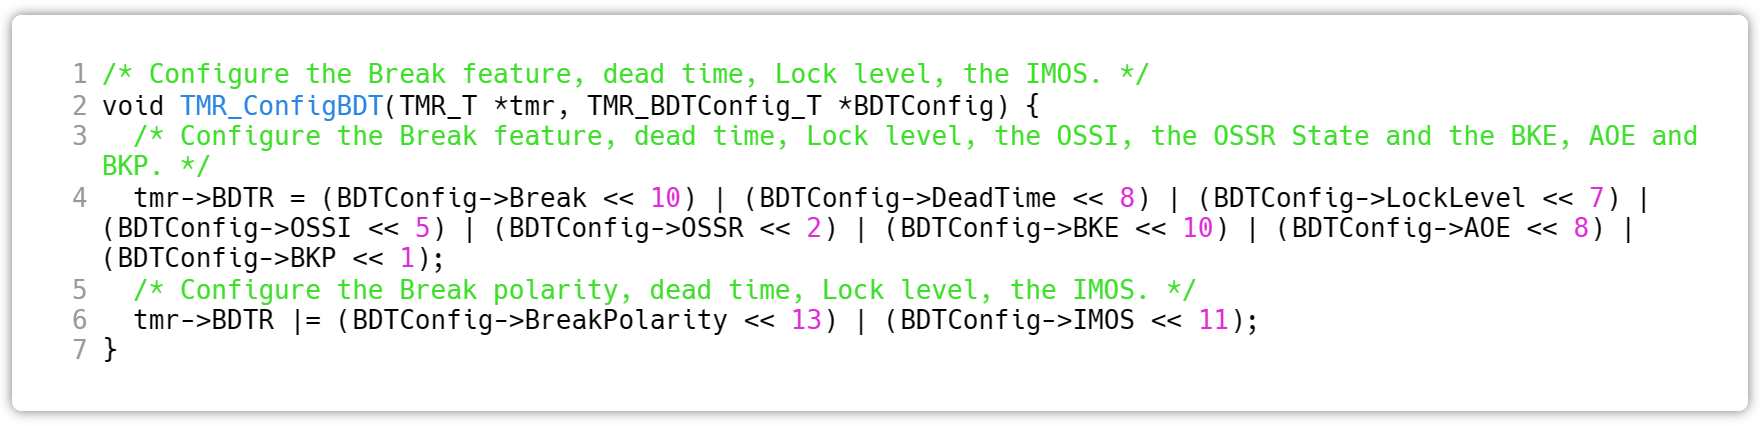
\includegraphics[width=1\textwidth]{obrazky/gpt3.png}
    \caption{Kód vygenerovaný nástrojom GitHub Copilot. Model bol inštruovaný, aby nakonfiguroval rôzne parametre, ako sú Break feature, dead time a Lock level. Výstup efektívne odráža tieto požiadavky.}
    \label{fig:gpt3}
\end{figure}


\section{MicoCoderFIM}

\begin{figure}[H]
    \centering
    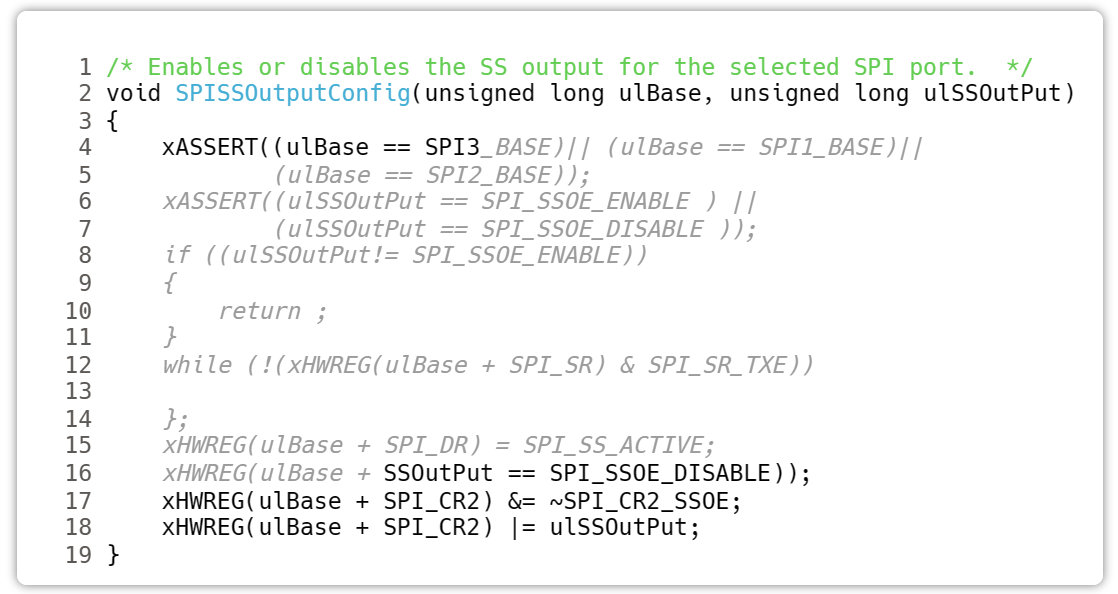
\includegraphics[width=0.8\textwidth]{obrazky/fim1.png}\\
    \caption{Výstup modelu \MCfim{}.}
    \label{fig:fim1}
\end{figure}

\begin{figure}[H]
    \centering
    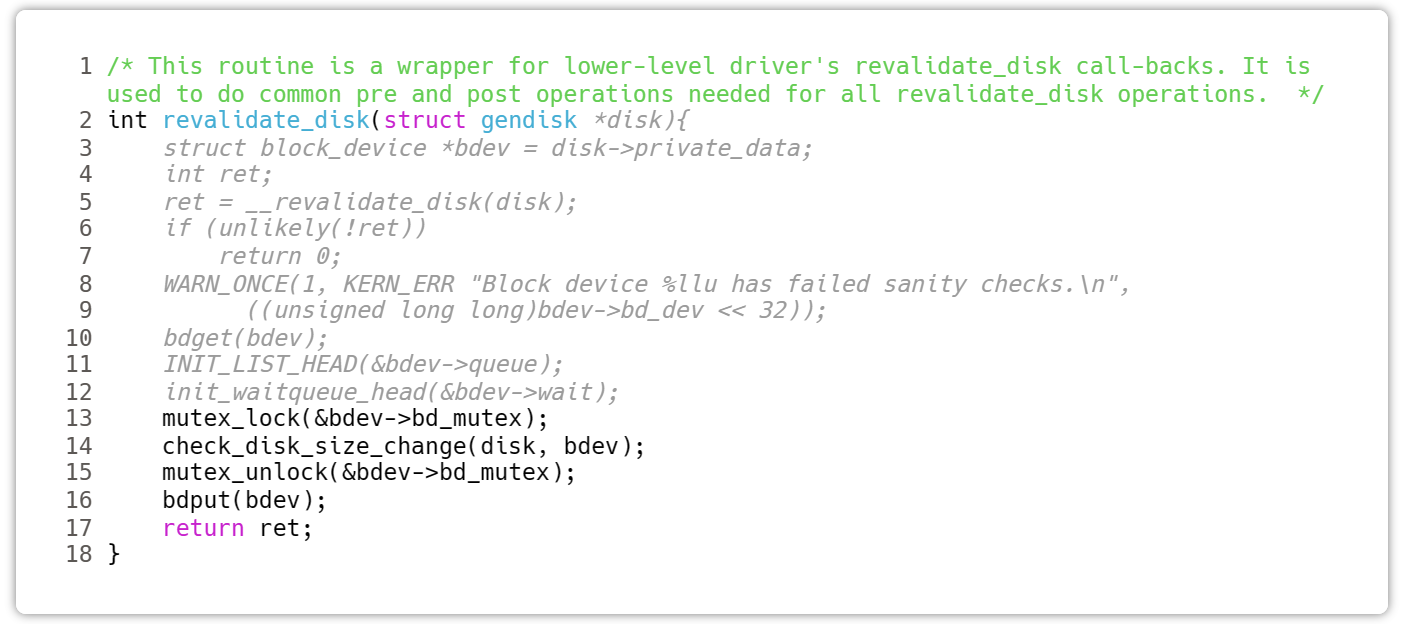
\includegraphics[width=0.8\textwidth]{obrazky/fim321.png}\\
    \caption{Výstup modelu \MCfim{}.}
    \label{fig:fim321}
\end{figure}

\begin{figure}[H]
    \centering
    \raisebox{-\height}{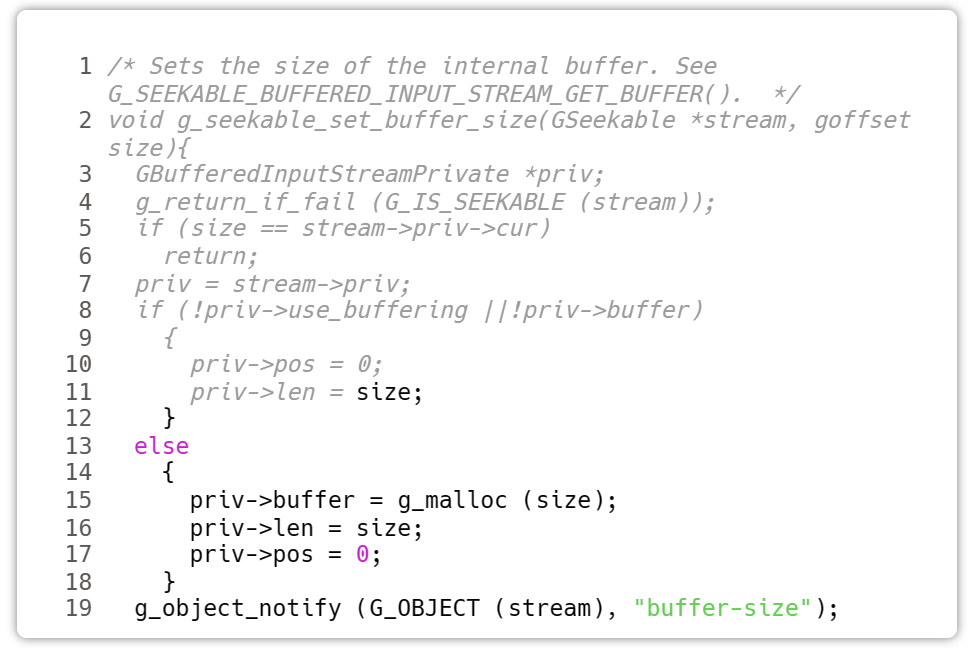
\includegraphics[width=0.45\textwidth]{obrazky/fim2.png}}
    \raisebox{-\height}{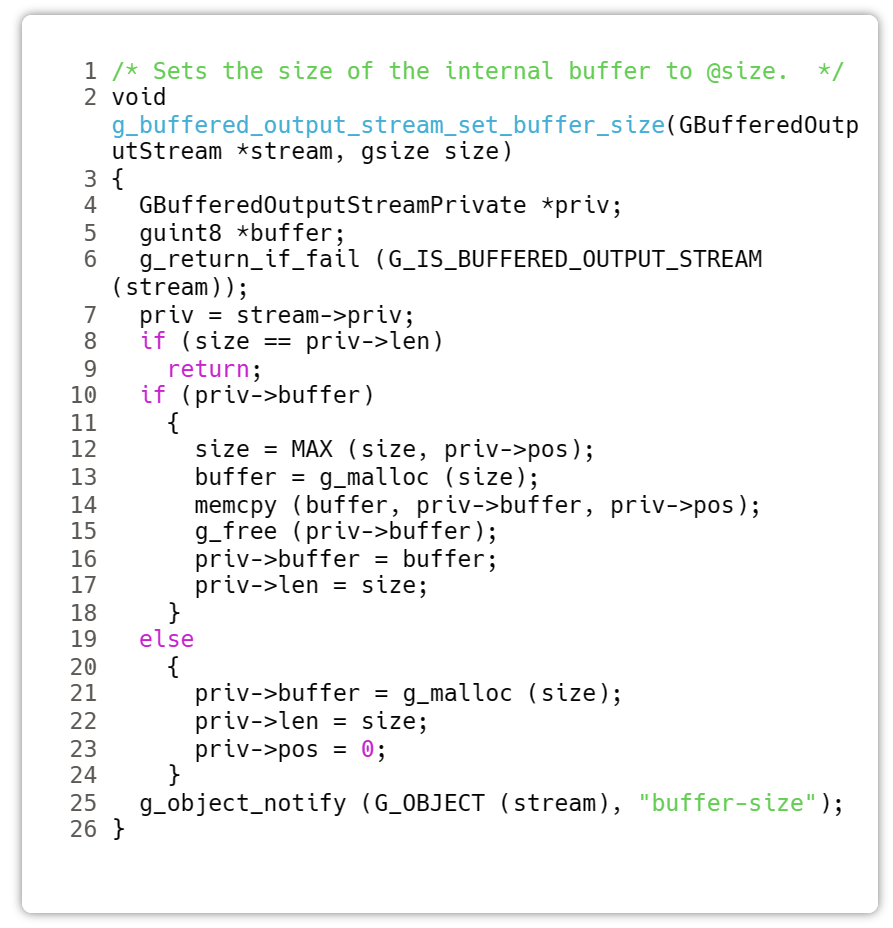
\includegraphics[width=0.45\textwidth]{obrazky/fim2ref.png}}
    \caption{Návrh kódu vygenerovaný modelom \MCfim{} (vľavo) a referenčné riešenie (vpravo).}
    \label{fig:fim2}
\end{figure}

\begin{figure}[H]
    \centering
    \raisebox{-\height}{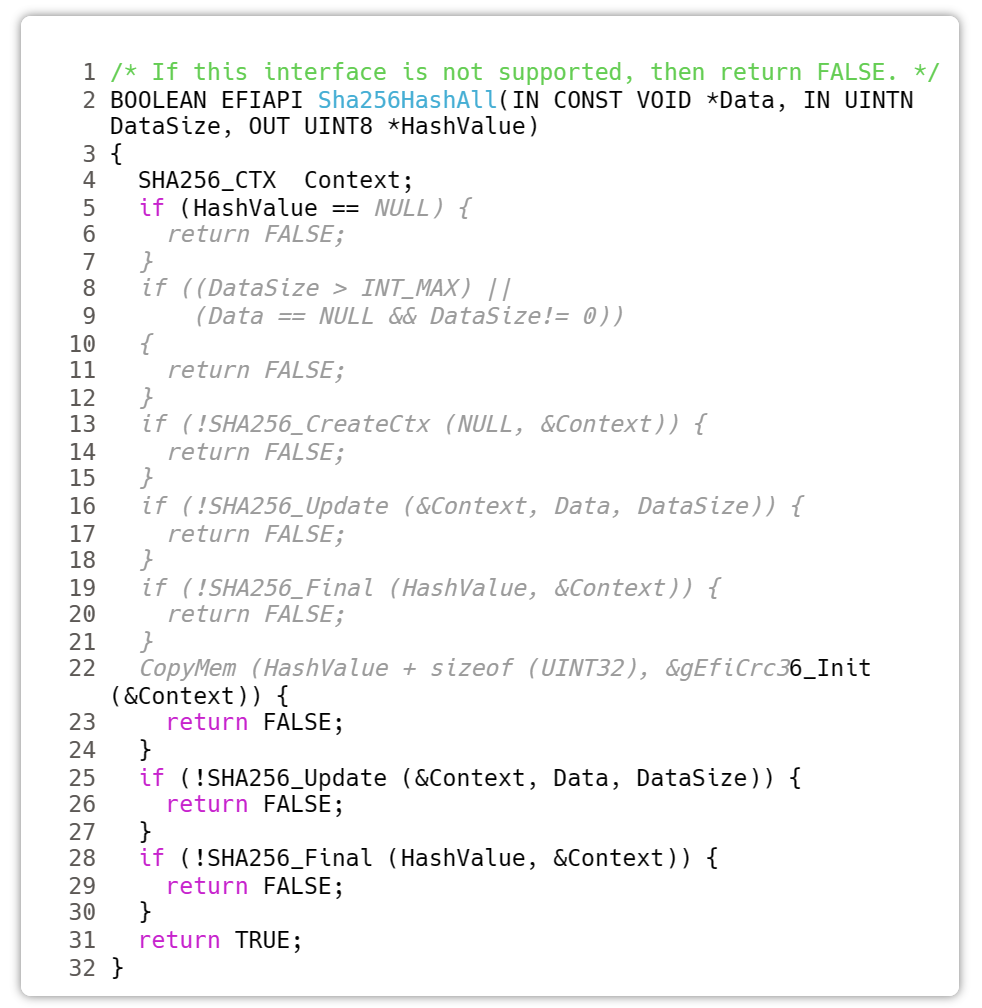
\includegraphics[width=0.45\textwidth]{obrazky/fim3.png}}
    \raisebox{-\height}{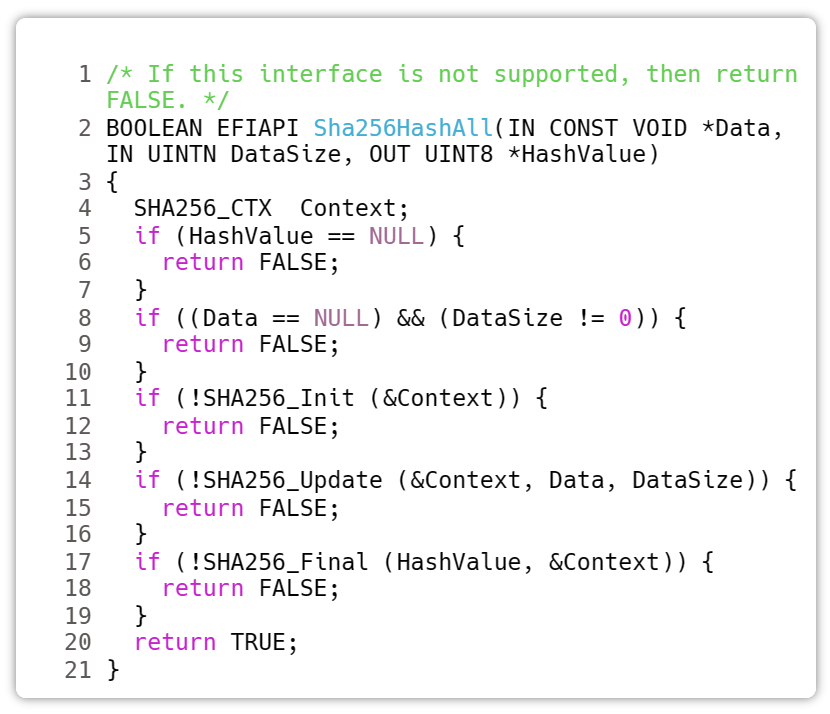
\includegraphics[width=0.45\textwidth]{obrazky/fim3ref.png}}
    \caption{Návrh kódu vygenerovaný modelom \MCfim{} (vľavo) a referenčné riešenie (vpravo).}
    \label{fig:fim3}
\end{figure}


\chapter{Výsledky modelu MicroCoderFIM pri rôznych nastaveniach}\label{app:fim_test}

Pre zistenie optimálnych nastavení parametrov teploty (temperature), maximálnej dĺžky generovanej sekvencie (max\_new\_tokens), a pravdepodobnosti výberu (top\_p), bola vykonaná sada experimentov na vzorke 250 príkladov. Analýza ukázala, že model dosahuje najlepšie celkové výsledky pri nastavení nižšej teploty (0.2 a 0.1) a  maximálnej dĺžke sekvencie 128 tokenov. Pre metriku CodeBLEU však model vykazoval lepšie výsledky pri dlhších sekvenciách (256 tokenov), čo naznačuje odlišnú dynamiku optimalizácie pre túto špecifickú metriku. Výsledky pre rôzne nastavenia teploty a maximálnej dĺžky generovanej sekvencie sú podrobne dokumentované v~grafoch, ktoré ilustrujú závislosti medzi meniacimi sa hodnotami týchto parametrov a výkonmi modelu. Hodnotenie parametru top\_p ukazuje, že model mal lepšie výsledky pri hodnote 0.5 ako pri 0.9, ale pri teplote 0.2 vykazuje najlepšie skóre. Podrobné výsledky sú na obrázku~\ref{fig:infer-test}.

Obrázok~\ref{fig:max-new-tokens} ukazuje, že obidva testy modelujú rovnaké chovanie nastavenia maximálnej dĺžky generovania. Pri nižších sekvenciách model vykazuje lepšie výsledky. Zároveň sa ukázalo, že pri metrike CodeBLEU dosahuje model o~takmer 10\% lepšie výsledky pri nastavení sekvencie 256 tokenov.

\begin{figure}
    \centering
    \includesvg[width=0.8\textwidth]{obrazky/temperature.svg}
    \includesvg[width=0.8\textwidth]{obrazky/top_p.svg}
    \caption{Výsledky inferencie modelu \MCfim{} pri rôznych nastaveniach teploty, top\_p a maximálnej dĺžky generovanej sekvencie. Model dosiahol najlepšie výsledky pri teplote 0.2 a maximálnej dĺžke 128 tokenov.}
    \label{fig:infer-test}
\end{figure}

\begin{figure}
    \centering
    \includesvg[width=0.8\textwidth]{obrazky/max_new_tokens.svg}
    \caption{Zmena výsledkov inferencie modelu \MCfim{} v~porovnaní so základným nastavením (128 tokenov) pri rôznych hodnotách maximálnej dĺžky generovanej sekvencie. Platí, že pri dĺžke 128 tokenov sa model správa lepšie v~troch metrikách. Metrika CodeBLEU vykazuje lepšie výsledky pri dĺžke 256 tokenov.}
    \label{fig:max-new-tokens}
\end{figure}